\section{Experimental Procedures}
We perform several experiments using the model "stable-diffusion-v1-5" by runwayml \cite{Rombach_2022_CVPR} and applying ToMe in different ways to a set of prompts and measuring the performance.
The performance is defined by\\ 
\(1)\) speed: the average diffusion time for every image of the set and\\
\(2)\) image quality: the FID-value between sets of images that had token merging applied and their counterparts (that is same prompt, seed and image size) that didn't use any token merging.



\subsection{Setup}
\subsubsection*{Creating image datasets}
The experiments always compare how diffusion time and image quality change across a spectrum of different volumes of tokens \((r)\) removed while token merging is applied in different layers of the transformer (self-attention, cross-attention and mlp).\\
The images were generated with a "DiffusionPipeline" from HuggingFace's diffusers library \cite{von-platen-etal-2022-diffusers}, using the \href{https://huggingface.co/runwayml/stable-diffusion-v1-5}{"stable-diffusion-v1-5"} model \cite{Rombach_2022_CVPR}.\\
We sampled multiple sets of 500 prompts from the dataset \href{https://huggingface.co/datasets/Gustavosta/Stable-Diffusion-Prompts}{"Stable-Diffusion-Prompts"} on HuggingFace which has 80,000 prompts filtered and extracted from the image finder for Stable Diffusion: \href{https://lexica.art}{Lexica.art}, and generated a corresponding set of random seeds.\\ 
Prompts appearing multiple times within a set was not specifically prevented, due to the extremely low probability of a specific prompt-seed-pair appearing multiple times within a dataset. Same prompts with different seeds result in different images and therefore do not corrupt the validity of a dataset by our assessment.\\
Multiple images were created per prompt, with a 0\%, 10\%, 20\%, 30\%, 40\%, 50\%, and 60\% (if possible) merge applied respectively, creating a set of 3,500 (or sometimes 3,000) images which can be split up into subsets of 500 images each for every merge volume.\\
---cfg scale? number diffusion steps?---



\subsubsection*{Measuring results}
For image quality, the FID between a subset with \(r > 0\%\) and the subset with \(r = 0\%\) of the same dataset is computed, to examine how ToMe performs with different values for \(r\).\\
The speed of image generation is assessed by recording the time taken to create each individual image and then calculating the average across all subsets.
\begin{lstlisting}[language=Python]
start = time.time()
image = pipeline(prompt, x, y, ...)
end = time.time()
time = end - start
\end{lstlisting}



\subsubsection*{Hardware}
All experiments were conducted with Nvidia GeForce GTX 1080 Ti GPUs. Individual images were always generated on a single GPU.



\subsection{Adjustments}
\subsubsection*{FID}
We created and used our own fork of pytorch-fid \cite{Seitzer2020FID} to accommodate for the hpc not being connected to the internet and therefore not being able to download the weights of the Inception model to calculate FID-values. Our version loads these weights from a local directory to avoid any connection to the internet and requires the user to have them pre-installed.



\subsubsection*{Prompts}
We shortened every prompt that exceeds 300 characters, in order to ensure that CLIP's token limit is not breached, as CLIP can only handle up to 77 tokens.
This is accomplished by determining the index (\(idx\)) of the last comma in the first 300 characters of every oversized prompt and then cutting off everything from this point onwards.
\begin{lstlisting}[language=Python]
prompt = prompt[:idx]
\end{lstlisting}


%\newpage
\subsection{Comparison to Original Setup}
\cite{bolya2023tomesd} structure their experiments as follows: "We use Stable diffusion v1.5 to generate 2,000 $512 \times 512$ images of ImageNet-1k \cite{deng2009imagenet} classes (2 per class) using 50 PLMS \cite{liu2022pseudo} diffusion steps with a cfg scale \cite{dhariwal2021diffusion} of 7.5. We then compute FID scores between those 2,000 samples and 5,000 class-balanced ImageNet-1k val examples using \cite{Seitzer2020FID}. To test speed, we simply average the time taken over all 2,000 samples on a single 4090 GPU."\\
\\
%\newpage
The most notable difference to our setup is that we compare a set of merged images with their own unmerged versions, while Bolya and Hoffman's approach compares image sets of the same categories but does not directly try to measure alterations of images created by ToMe.\\
Additionally, Bolya and Hoffman also measured and analyzed the memory usage during the diffusion process, while we left memory consumption completely out of the scope of this work.



%\newpage
\subsection{Results}
The baseline is to look at the effects of ToMe (with default settings) applied to $768 \times 768$ images. The experiments can be split up into three different parts inspecting how ToMe affects performance\\ \(1)\) when applied to different parts of the transformer,\\ \(2)\) when applied to smaller $512 \times 512$ images, and\\ \(3)\) when different settings for partitioning the \textbf{src} and \textbf{dst} sets are used.\\
\\
The results of every experimental unit are presented in two figures. The first figure focuses on image quality, displaying FID values, while the subsequent one emphasizes image generation speed by showcasing how the average time required for image generation of each subset compares to the \(r=0\%\) subset.
Both figures have \(r\%\) on the x-axis showing how the metrics change with an increasing amount of tokens merged.

\subsubsection*{1): Experimenting with different components of the transformer}
ToMe's default configuration involves token merging solely within the self-attention module.
Our experiment aims to gauge how the performance metrics are affected by extending token merging to different combinations of transformer components.\\
All image sets were created with the same set of prompts and seeds (unless stated otherwise) to ensure the comparability of the results.



\subsubsection*{1.1): default (only self-attn) vs all (self-attn, cross-attn and mlp)}
The first experiment of part 1 compares the default setting of ToMe where token merging is only applied in the self-attn layer (black) with a different configuration that has token merging applied in the self-attn, cross-attn and mlp layer (red). 
The naive idea here is to improve performance by using token merging in every transformer layer.
\begin{figure}[!htb]
\label{fig:exp_1_1}
   % FID values for run2 and run3
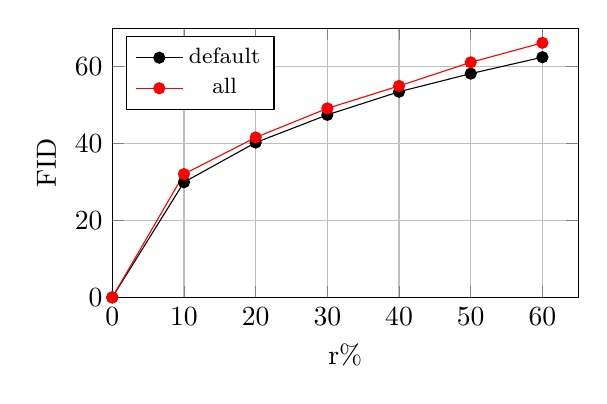
\begin{tikzpicture}
\begin{axis}[
    title={},
    height=5cm,
    width=7.5cm,
    xlabel={r\%},
    ylabel={FID},
    xmin=0, xmax=65,
    ymin=0, ymax=70,
    xtick={0,10,20,30,40,50,60},
    ytick={0,20,40,60},
    legend pos=north west,
    xmajorgrids=true,
    ymajorgrids=true,
    legend style={font=\footnotesize}
]

\addplot[
    color=black,
    mark=*
    ]
    coordinates {
    (0,0)(10,29.95)(20,40.26)(30,47.47)(40,53.48)(50,58.19)(60,62.46)
    };
    
\addplot[
    color=red,
    mark=*
    ]
    coordinates {
    (0,0)(10,32.07)(20,41.60)(30,49.15)(40,54.99)(50,61.13)(60,66.20)
    };
    
\legend{default, all}
    
\end{axis}
\end{tikzpicture}
   % time values for run2 and run3
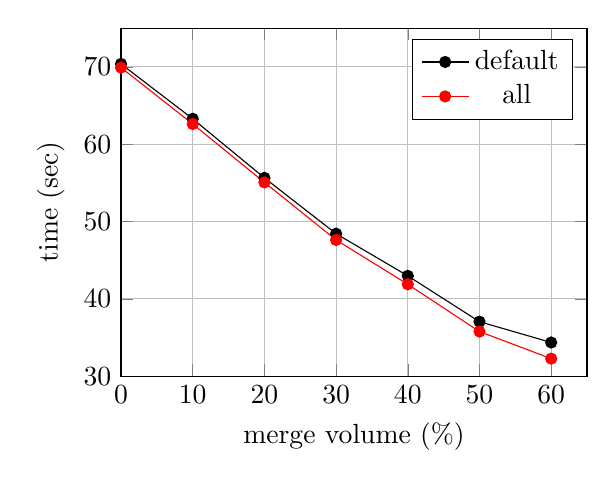
\begin{tikzpicture}
\begin{axis}[
    title={},
    height=6cm,
    width=7.5cm,
    xlabel={merge volume (\%)},
    ylabel={time (sec)},
    xmin=0, xmax=65,
    ymin=30, ymax=75,
    xtick={0,10,20,30,40,50,60},
    ytick={30,40,50,60,70},
    legend pos=north east,
    xmajorgrids=true,
    ymajorgrids=true,
]

\addplot[
    color=black,
    mark=*
    ]
    coordinates {
    (0,70.38)(10,63.28)(20,55.64)(30,48.42)(40,42.97)(50,37.04)(60,34.35)
    };
    
\addplot[
    color=red,
    mark=*
    ]
    coordinates {
    (0,69.91)(10,62.61)(20,55.06)(30,47.61)(40,41.88)(50,35.76)(60,32.26)
    };
    
\legend{default, all}
    
\end{axis}
\end{tikzpicture}
\caption{FID and relative time compared to r=0\% for 1.1)}
\label{fig:exp_1_1}
\end{figure}\\
%\newpage
This seemingly does not yield significant improvements as image generation speed does narrowly decrease by up to 2.1 s/im (this time-delta is below 1 s/im for $r<40\%$ though; see Tab.~\ref{table:exp_1_1}), albeit at a clear cost of image quality with FID being consistently larger for this configuration. \\
ToMe in its default setup consistently produces images closer to their no-ToMe original (see Fig.~\ref{fig:exp_1_1}), so extending token merging to both the cross-attn and mlp layer does not appear beneficial. This naive approach can therefore be disregarded.



%\newpage
\subsubsection*{1.2): [default] vs [self-attn \& cross-attn] vs [self-attn \& mlp]}
After \(1.1\), the question remains whether performance drops were caused by using ToMe in both the cross-attn and mlp layer or only one of them, so the second experiment of part 1 attempts to delve deeper into that matter. This time token merging is only extended to either the cross-attn (red) or the mlp module (blue). Then a comparison is made with the results of the default ToMe settings (black) from the previous trial.
\begin{figure}[!htb]
    % FID values for run2, run4 and run5
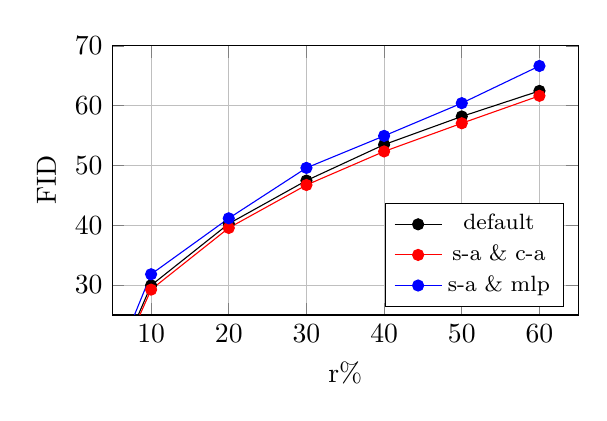
\begin{tikzpicture}
\begin{axis}[
    title={},
    height=5cm,
    width=7.5cm,
    xlabel={r\%},
    ylabel={FID},
    xmin=5, xmax=65,
    ymin=25, ymax=70,
    xtick={10,20,30,40,50,60},
    ytick={30,40,50,60,70},
    legend pos=south east,
    xmajorgrids=true,
    ymajorgrids=true,
    legend style={font=\footnotesize}
]

\addplot[
    color=black,
    mark=*
    ]
    coordinates {
    (0,0)(10,29.95)(20,40.26)(30,47.47)(40,53.48)(50,58.19)(60,62.46)
    };
    
\addplot[
    color=red,
    mark=*
    ]
    coordinates {
    (0,0)(10,29.24)(20,39.55)(30,46.73)(40,52.34)(50,57.05)(60,61.64)
    };

\addplot[
    color=blue,
    mark=*
    ]
    coordinates {
    (0,0)(10,31.81)(20,41.16)(30,49.59)(40,54.94)(50,60.41)(60,66.63)
    };
    
\legend{default, s-a \& c-a, s-a \& mlp}
    
\end{axis}
\end{tikzpicture}
    % time values for run2, run4 and run5
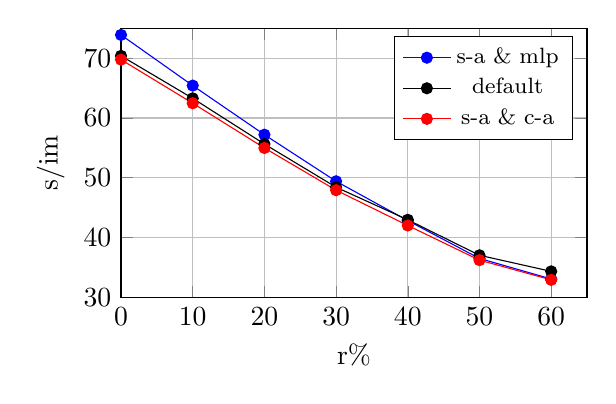
\begin{tikzpicture}
\begin{axis}[
    title={},
    height=5cm,
    width=7.5cm,
    xlabel={r\%},
    ylabel={s/im},
    xmin=0, xmax=65,
    ymin=30, ymax=75,
    xtick={0,10,20,30,40,50,60},
    ytick={30,40,50,60,70},
    legend pos=north east,
    xmajorgrids=true,
    ymajorgrids=true,
    legend style={font=\footnotesize}
]

\addplot[
    color=blue,
    mark=*
    ]
    coordinates {
    (0,73.88)(10,65.41)(20,57.20)(30,49.41)(40,42.83)(50,36.51)(60,33.08)
    };

\addplot[
    color=black,
    mark=*
    ]
    coordinates {
    (0,70.38)(10,63.28)(20,55.64)(30,48.42)(40,42.97)(50,37.04)(60,34.35)
    };
    
\addplot[
    color=red,
    mark=*
    ]
    coordinates {
    (0,69.75)(10,62.46)(20,54.98)(30,47.92)(40,42.02)(50,36.23)(60,32.93)
    };

    
\legend{s-a \& mlp, default, s-a \& c-a}
    
\end{axis}
\end{tikzpicture}
\caption{FID and relative time compared to r=0\% for 1.2)}
\label{fig:exp_1_2}
\end{figure}\\
%\newpage
This time it's clearly visible that merging tokens within the self-attn and cross-attn module performs the best, both in terms of image quality and image generation speed, notably surpassing the default configuration established by Bolya and Hofmann (see Fig.~\ref{fig:exp_1_2}).\\
Token merging in the self-attn and mlp module on the other hand noticeably worsens the image quality across the board as well as the generation speed when $r<40\%$ compared to the default (see Tab.~\ref{table:exp_1_2}).\\
We can therefore conclude that extending token merging to the cross-attn module has positive effects on the performance, while extending it to the mlp module has the opposite effect.



%\newpage
\subsubsection*{1.3): [default] vs [cross-attn \& mlp] vs [only cross-attn]}
The common denominator of the previous examinations was the application of token merging in the self-attn layer. This time we are explicitly avoiding token merging in the self-attn module and instead apply it in only the cross-attn (blue) and both the cross-attn and mlp component (red).
The results of the default ToMe settings (black) again carry over from the previous trial.\\
\begin{figure}[!htb]
    % FID values for run2, run6 and run7
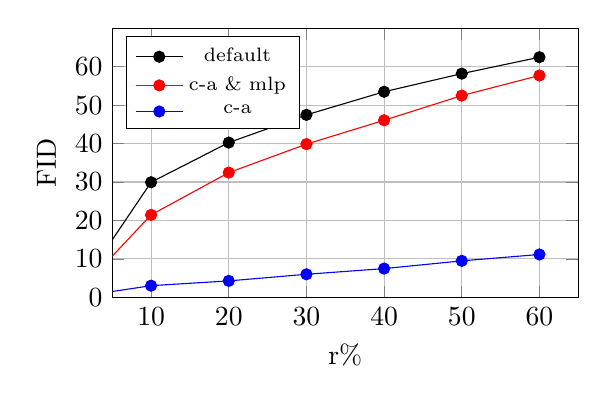
\begin{tikzpicture}
\begin{axis}[
    title={},
    height=5cm,
    width=7.5cm,
    xlabel={r\%},
    ylabel={FID},
    xmin=5, xmax=65,
    ymin=0, ymax=70,
    xtick={10,20,30,40,50,60},
    ytick={0,10,20,30,40,50,60},
    legend pos=north west,
    xmajorgrids=true,
    ymajorgrids=true,
    legend style={font=\scriptsize}
]

\addplot[
    color=black,
    mark=*
    ]
    coordinates {
    (0,0)(10,29.95)(20,40.26)(30,47.47)(40,53.48)(50,58.19)(60,62.46)
    };
    
\addplot[
    color=red,
    mark=*
    ]
    coordinates {
    (0,0)(10,21.46)(20,32.45)(30,39.86)(40,46.06)(50,52.48)(60,57.71)
    };

\addplot[
    color=blue,
    mark=*
    ]
    coordinates {
    (0,0)(10,3.05)(20,4.29)(30,6.01)(40,7.49)(50,9.50)(60,11.16)
    };

    
\legend{default, c-a \& mlp, c-a}
    
\end{axis}
\end{tikzpicture}
    % time values for run10 and run11
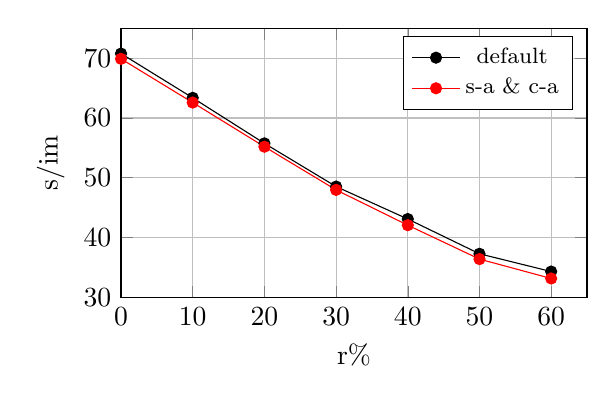
\begin{tikzpicture}
\begin{axis}[
    title={},
    height=5cm,
    width=7.5cm,
    xlabel={r\%},
    ylabel={s/im},
    xmin=0, xmax=65,
    ymin=30, ymax=75,
    xtick={0,10,20,30,40,50,60},
    ytick={30,40,50,60,70},
    legend pos=north east,
    xmajorgrids=true,
    ymajorgrids=true,
    legend style={font=\footnotesize}
]

\addplot[
    color=black,
    mark=*
    ]
    coordinates {
    (0,70.76)(10,63.36)(20,55.75)(30,48.53)(40,43.10)(50,37.29)(60,34.32)
    };
    
\addplot[
    color=red,
    mark=*
    ]
    coordinates {
    (0,69.88)(10,62.57)(20,55.19)(30,47.97)(40,42.07)(50,36.40)(60,33.16)
    };
    
\legend{default, s-a \& c-a}
    
\end{axis}
\end{tikzpicture}
\caption{FID and relative time compared to r=0\% for 1.3)}
\label{fig:exp_1_3}
\end{figure}\\
The most striking result here is that no token merging in the self-attn layer corresponds to no image generation speedup at all, rather slowing the process down (see Tab.~\ref{table:exp_1_3}). 
The apparent improvements to image quality compared to the ToMe default (see Fig.~\ref{fig:exp_1_3}) consequently become negligible without any speed benefits, though it can be noted that token merging in only the cross-attn layer greatly outperforms token merging in both cross-attn and mlp layer in terms of image quality.\\
We conclusively derive that ToMe without involvement of the self-attn layer does not accelerate the image generation process at all and can be considered redundant and therefore be disregarded. It can additionally be derived from \(1.1 - 1.3\) that token merging in the mlp layer has strong negative effects on image quality.




%\newpage
\subsubsection*{1.4): [default] vs [self-attn \& cross-attn] (the second time)}
The most prominent takeaway of the first three experiments is that token merging in both the self-attn and cross-attn layers improves the performance of ToMe both in terms of image quality and image generation speed.\\
We want to further examine this discovery by repeating the experiment with a new set of 500 different prompt-seed pairs and then average the results of both trials.
\begin{figure}[!htb]
    % FID values for run8 and run9
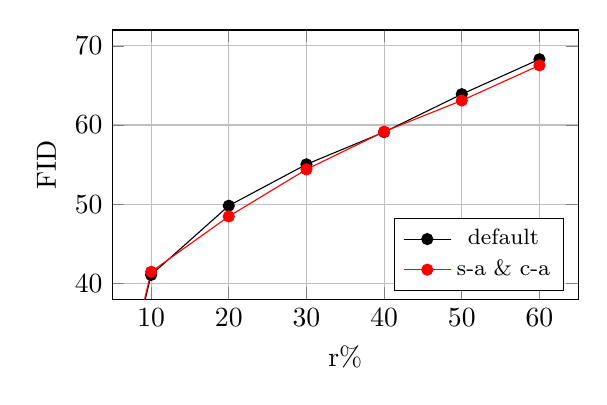
\begin{tikzpicture}
\begin{axis}[
    title={},
    height=5cm,
    width=7.5cm,
    xlabel={r\%},
    ylabel={FID},
    xmin=5, xmax=65,
    ymin=38, ymax=72,
    xtick={10,20,30,40,50,60},
    ytick={30,40,50,60,70},
    legend pos=south east,
    xmajorgrids=true,
    ymajorgrids=true,
    legend style={font=\footnotesize}
]

\addplot[
    color=black,
    mark=*
    ]
    coordinates {
    (0,0)(10,41.06)(20,49.80)(30,55.03)(40,59.10)(50,63.89)(60,68.30)
    };
    
\addplot[
    color=red,
    mark=*
    ]
    coordinates {
    (0,0)(10,41.45)(20,48.45)(30,54.39)(40,59.16)(50,63.09)(60,67.53)
    };
    
\legend{default, s-a \& c-a}
    
\end{axis}
\end{tikzpicture}
    % time values for run8 and run9
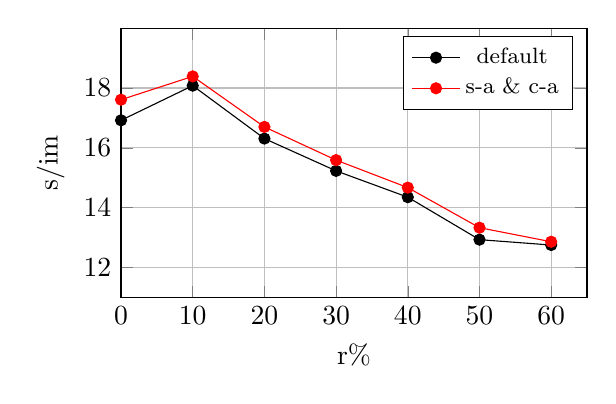
\begin{tikzpicture}
\begin{axis}[
    title={},
    height=5cm,
    width=7.5cm,
    xlabel={r\%},
    ylabel={s/im},
    xmin=0, xmax=65,
    ymin=11, ymax=20,
    xtick={0,10,20,30,40,50,60},
    ytick={12,14,16,18},
    legend pos=north east,
    xmajorgrids=true,
    ymajorgrids=true,
    legend style={font=\footnotesize}
]

\addplot[
    color=black,
    mark=*
    ]
    coordinates {
    (0,16.92)(10,18.08)(20,16.31)(30,15.23)(40,14.35)(50,12.93)(60,12.75)
    };
    
\addplot[
    color=red,
    mark=*
    ]
    coordinates {
    (0,17.61)(10,18.39)(20,16.70)(30,15.59)(40,14.67)(50,13.33)(60,12.86)
    };
    
\legend{default, s-a \& c-a}
    
\end{axis}
\end{tikzpicture}
\caption{FID and relative time compared to r=0\% for 1.4)}
\label{fig:exp_1_4}
\end{figure}\\
%\newpage
It is again clearly visible that token merging only in the self-attn module (black) is outperformed by expanding it to the cross-attn module (red) as well (see Fig.~\ref{fig:exp_1_4}). This improvement consistently appears with every \(r\), with the gap slightly widening for larger values of \(r\) (see Tab.~\ref{table:exp_1_4}).\\
This motivates the use of token merging in both the self-attn and cross-attn modules as the new default for $768 \times 768$ images going forward.



%\newpage
\subsubsection*{2): Exploring smaller images sizes}
In this section, we want to expand the scope of our trials to smaller image sizes. Precisely, we want to repeat looking at token merging in the self-attn layer (black) and both the self-attn and cross-attn layer (red), but this time with smaller $512 \times 512$ images. Again a set of 500 prompts is randomly sampled and a corresponding set of random seeds is generated.
\begin{figure}[!htb]
    % FID values for run8 and run9
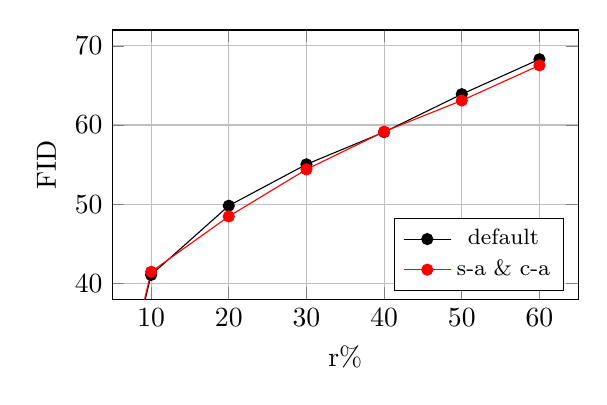
\begin{tikzpicture}
\begin{axis}[
    title={},
    height=5cm,
    width=7.5cm,
    xlabel={r\%},
    ylabel={FID},
    xmin=5, xmax=65,
    ymin=38, ymax=72,
    xtick={10,20,30,40,50,60},
    ytick={30,40,50,60,70},
    legend pos=south east,
    xmajorgrids=true,
    ymajorgrids=true,
    legend style={font=\footnotesize}
]

\addplot[
    color=black,
    mark=*
    ]
    coordinates {
    (0,0)(10,41.06)(20,49.80)(30,55.03)(40,59.10)(50,63.89)(60,68.30)
    };
    
\addplot[
    color=red,
    mark=*
    ]
    coordinates {
    (0,0)(10,41.45)(20,48.45)(30,54.39)(40,59.16)(50,63.09)(60,67.53)
    };
    
\legend{default, s-a \& c-a}
    
\end{axis}
\end{tikzpicture}
    % time values for run2, run6 and run7
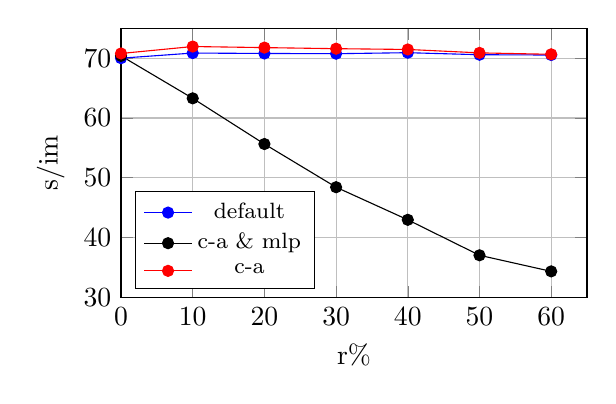
\begin{tikzpicture}
\begin{axis}[
    title={},
    height=5cm,
    width=7.5cm,
    xlabel={r\%},
    ylabel={s/im},
    xmin=0, xmax=65,
    ymin=30, ymax=75,
    xtick={0,10,20,30,40,50,60},
    ytick={30,40,50,60,70},
    legend pos=south west,
    xmajorgrids=true,
    ymajorgrids=true,
    legend style={font=\footnotesize}
]

\addplot[
    color=blue,
    mark=*
    ]
    coordinates {
    (0,69.99)(10,70.85)(20,70.78)(30,70.74)(40,70.91)(50,70.57)(60,70.52)
    };

\addplot[
    color=black,
    mark=*
    ]
    coordinates {
    (0,70.38)(10,63.28)(20,55.64)(30,48.42)(40,42.97)(50,37.04)(60,34.35)
    };
    
\addplot[
    color=red,
    mark=*
    ]
    coordinates {
    (0,70.78)(10,71.94)(20,71.76)(30,71.58)(40,71.45)(50,70.88)(60,70.64)
    };

    
\legend{default, c-a \& mlp, c-a}
    
\end{axis}
\end{tikzpicture}
\caption{FID and relative time compared to r=0\% for 2)}
\label{fig:exp_2}
\end{figure}\\
%\newpage
The success of \(1.4\) does not repeat, as this time it was consistently slower to create images with token merging in the cross-attn block (see Fig.~\ref{fig:exp_2}). The FID seems to bounce a bit with the default performing slightly better for \(r=10\%\) and \(r=40\%\), but performing worse the rest of the time (see Tab.~\ref{table:exp_2}). \\
The overall speed gains are considerably smaller compared to the \(768 \times 768\) images. Even at \(r=60\%\), the speed gain is only about 25\% and the image generation process actually becomes slower by about 1 s/im at \(r=10\%\) (see Tab.~\ref{table:exp_2}).\\
We conclude that using ToMe for such small images (e.g. $512 \times 512$ or smaller) is less practical than it is for larger images. It is especially inadvisable to be used with a small merge volume (\(r<20\%\)), as there is no time gained in the diffusion process, but information is nonetheless lost during merging. \\
In consequence, we will not investigate the usage of ToMe on this scale any further. Neither will we investigate ToMe's effect on larger images due to hardware limitations.



%\newpage
\subsubsection*{3): Exploring different batch sizes}
The third part of the experimental section examines, how different values for \(sx\) and \(sy\) influence the performance of ToMe on $768 \times 768$ images. As a reminder, \(sx\) and \(sy\) determine the size of the token batches, which are used to spread the \textbf{dst} tokens somewhat evenly across the image, with larger batches resulting in a less consistent distribution. Our new default of ToMe with token merging applied in both the self-attn and cross-attn layer will be used throughout this section.



%\newpage
\subsubsection*{3.1): $3 \times 3$ batches}
The first choice was scaling up from $2 \times 2$ (black) to $3 \times 3$ batches (red). This setup strongly tilts the ratio of src and dst tokens toward the former and theoretically allows for a larger number of tokens to be merged. 
\begin{align*}
    r_{max} = 1-\frac{1}{3*3} = \frac{8}{9} \approx 88.89\%
\end{align*}
We will, nevertheless, not exceed a merge rate of \(r=60\%\), as image quality already exhibits clear deterioration at that level and also due to the absence of other data available for comparison.



\subsubsection*{3.2): $1 \times 2$ vertical batches}
Scaling down the same way to $1 \times 1$ batches is impossible, as it would result in every token landing in the \textbf{dst} set and \(r_{max}=0\%\).\\
We therefore chose to cut the batches in half horizontally, creating $1 \times 2$ batches. This decision led to a balanced 50-50 distribution between \textbf{src} and \textbf{dst}.
\begin{align*}
    r_{max} = 1-\frac{1}{1*2} = 50\%
\end{align*}
This limits our merge volume to 50\% but allows for better matches during the merge process. Compared to the $2 \times 2$ default, every \textbf{src} token now has double the number of \textbf{dst} tokens to be matched with.\\
\begin{figure}[!htb]
    % FID values for run11, run14 and run15 
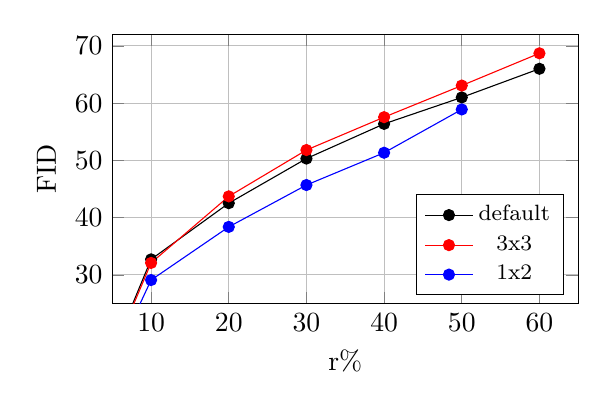
\begin{tikzpicture}
\begin{axis}[
    title={},
    height=5cm,
    width=7.5cm,
    xlabel={r\%},
    ylabel={FID},
    xmin=5, xmax=65,
    ymin=25, ymax=72,
    xtick={10,20,30,40,50,60},
    ytick={30,40,50,60,70},
    legend pos=south east,
    xmajorgrids=true,
    ymajorgrids=true,
    legend style={font=\footnotesize}
]

\addplot[
    color=black,
    mark=*
    ]
    coordinates {
    (0,0)(10,32.71)(20,42.52)(30,50.31)(40,56.37)(50,60.99)(60,65.99)
    };
    
\addplot[
    color=red,
    mark=*
    ]
    coordinates {
    (0,0)(10,32.09)(20,43.71)(30,51.80)(40,57.54)(50,63.06)(60,68.69)
    };

\addplot[
    color=blue,
    mark=*
    ]
    coordinates {
    (0,0)(10,29.10)(20,38.38)(30,45.69)(40,51.33)(50,58.89)
    };
    
\legend{default, 3x3, 1x2}
    
\end{axis}
\end{tikzpicture}
    % time values for run11, run14 and run15
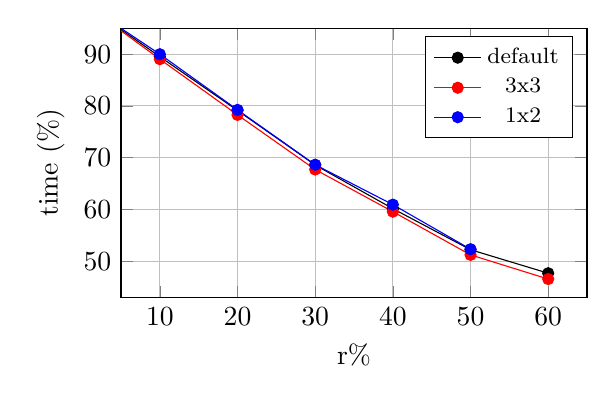
\begin{tikzpicture}
\begin{axis}[
    title={},
    height=5cm,
    width=7.5cm,
    xlabel={r\%},
    ylabel={time (\%)},
    xmin=5, xmax=65,
    ymin=43, ymax=95,
    xtick={10,20,30,40,50,60},
    ytick={50,60,70,80,90},
    legend pos=north east,
    xmajorgrids=true,
    ymajorgrids=true,
    legend style={font=\footnotesize}
]

\addplot[
    color=black,
    mark=*
    ]
    coordinates {
    (0,100)(10,89.50)(20,79.11)(30,68.57)(40,60.14)(50,52.21)(60,47.67)
    };
    
\addplot[
    color=red,
    mark=*
    ]
    coordinates {
    (0,100)(10,89.02)(20,78.26)(30,67.70)(40,59.56)(50,51.21)(60,46.54)
    };

\addplot[
    color=blue,
    mark=*
    ]
    coordinates {
    (0,100)(10,89.98)(20,79.23)(30,68.63)(40,60.92)(50,52.31)
    };
    
\legend{default, 3x3, 1x2}
    
\end{axis}
\end{tikzpicture}
\caption{FID and relative time compared to r=0\% for 3)}
\label{fig:exp_3}
\end{figure}\\
The resizing of the batches has only minor effects on image generation speed, as all three configurations consistently remain within one second of each other (see Tab.~\ref{table:exp_3}).\\
Image quality shows a noticeable improvement with decreasing batch sizes. The ToMe version with $3 \times 3$ batches is slightly surpassed by the $2 \times 2$ version, and this improvement is further enhanced when transitioning to $1 \times 2$ batches. (see Fig.~\ref{fig:exp_3}).
The gap closes towards \(r=50\%=r_{max}\), as every \textbf{src} token has to be merged when using $1 \times 2$ batches, regardless of how good of a match from \textbf{dst} is available.\\
It can still be concluded that using the $1 \times 2$ batches to create an equal number of \textbf{src} and \textbf{dst} tokens yields the best performance, especially when \(r\) is not close to \(0\%\) or \(r_{max}\), while the usage of larger batches with a smaller \(\textbf{dst\%}\) is not advisable.



%\newpage
\subsubsection*{4): Putting it all together}
Finally, we are comparing the most successful configurations from the past experiments. That means we are looking at \textbf{setup 1}: the ToMe default by Bolya and Hofmann (black), \textbf{setup 2}: our new default with token merging expanded to the cross-attn layer from \(1.2\) and \(1.4\) (red), and \textbf{setup 3}: the new default but with $1 \times 2$ batches for token partitioning from \(3.2\) (blue).\\
We expanded the image sets for the first two configurations to 1000 images per merge volume in \(1.4\), so we will do the same for the other one to enable examinations on a larger scale.
\begin{figure}[!htb]
    % FID values for run2/10, run4/11 and run15/16
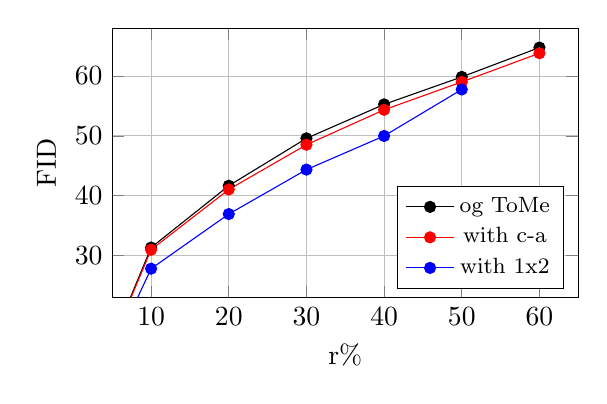
\begin{tikzpicture}
\begin{axis}[
    title={},
    height=5cm,
    width=7.5cm,
    xlabel={r\%},
    ylabel={FID},
    xmin=5, xmax=65,
    ymin=23, ymax=68,
    xtick={10,20,30,40,50,60},
    ytick={30,40,50,60},
    legend pos=south east,
    xmajorgrids=true,
    ymajorgrids=true,
    legend style={font=\footnotesize}
]

\addplot[
    color=black,
    mark=*
    ]
    coordinates {
    (0,0)(10,31.33)(20,41.67)(30,49.59)(40,55.27)(50,59.86)(60,64.77)
    };
    
\addplot[
    color=red,
    mark=*
    ]
    coordinates {
    (0,0)(10,30.97)(20,41.04)(30,48.52)(40,54.36)(50,59.02)(60,63.82)
    };

\addplot[
    color=blue,
    mark=*
    ]
    coordinates {
    (0,0)(10,27.80)(20,36.93)(30,44.36)(40,49.99)(50,57.76)
    };
    
\legend{og ToMe, with c-a, with 1x2}
    
\end{axis}
\end{tikzpicture}
    % time values for run2/10, run4/11, run15/16
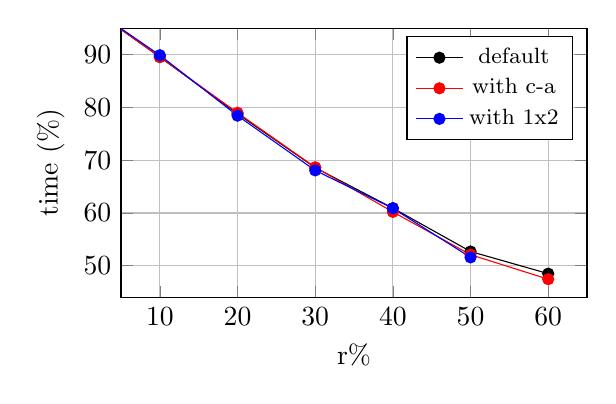
\begin{tikzpicture}
\begin{axis}[
    title={},
    height=5cm,
    width=7.5cm,
    xlabel={r\%},
    ylabel={time (\%)},
    xmin=5, xmax=65,
    ymin=44, ymax=95,
    xtick={10,20,30,40,50,60},
    ytick={50,60,70,80,90},
    legend pos=north east,
    xmajorgrids=true,
    ymajorgrids=true,
    legend style={font=\footnotesize}
]

\addplot[
    color=black,
    mark=*
    ]
    coordinates {
    (0,100)(10,89.54)(20,78.79)(30,68.58)(40,60.91)(50,52.70)(60,48.50)
    };
    
\addplot[
    color=red,
    mark=*
    ]
    coordinates {
    (0,100)(10,89.54)(20,78.98)(30,68.65)(40,60.20)(50,52.09)(60,47.45)
    };

\addplot[
    color=blue,
    mark=*
    ]
    coordinates {
    (0,100)(10,89.89)(20,78.43)(30,68.06)(40,60.88)(50,51.58)
    };
    
\legend{default, with c-a, with 1x2}
    
\end{axis}
\end{tikzpicture}
\caption{FID and relative time compared to r=0\% for 4)}
\label{fig:exp_4}
\end{figure}\\
Again, speed is very close across the board, as \textbf{setup 2} is the fastest by only a small margin (see Tab.~\ref{table:exp_4}).
Our discoveries regarding image quality are also reinforced, with \textbf{setup 3} noticeably outperforming the rest and \textbf{setup 1} consistently being the worst (see Fig.~\ref{fig:exp_4}).\\



%\newpage
\subsubsection*{Summary}
The experiments we conducted suggest that the best performance can be achieved by applying token merging in both the self-attn and cross-attn layer of the transformer. Depending on whether speed or image quality is the most important demand, $1 \times 2$ (best image quality) or $2 \times 2$ batches (highest speed) can be chosen for token partitioning, with $1 \times 2$ batches bringing particularly great improvements to image quality when \(r\leq40\%\).\\
Another important discovery is that token merging in the self-attn module is essential to unlocking speed improvements for image generation. On the other hand, using ToMe in the mlp layer seems to exclusively come at a disadvantage.\\
Moreover, it is important to create sufficiently large images when using ToMe in order to see the speed benefits. We showed that the time improvements with token merging noticeably decrease from >50\% for $768 \times 768$ images to only about 25\% for $512 \times 512$ images at \(r=60\%\) (see Tab.~\ref{table:exp_1_4},~\ref{table:exp_2}).\\
Additionally, it was shown that strongly skewing the \textbf{src}-\textbf{dst}-ratio away from an equal distribution has negative effects on image quality as well (see Tab.~\ref{table:exp_2}).




%\newpage
\subsection{Comparison to Original Results}
The great differences in experimental setups and hardware make it impossible to compare specific numbers. The general promises of ToMe for SD by Bolya and Hofmann can be confirmed though, as our results show that ToMe makes image generation up to $2 \times$ faster while still maintaining great image quality at \(r = 60\%\).\\
\\
However, our findings suggest different configurations of ToMe yield better results.
Firstly, we found out that expanding token merging from only the self-attn layer to the cross-attn layer improves both speed and quality. There was no data for this setup listed by Bolya and Hofmann, although they mentioned: "Note that FID does not consider prompt adherence, which is likely why merging the cross-attn module actually reduces FID" \cite{bolya2023tomesd}. \\
The implicit assertion that extending token merging to the cross-attn module lowers image quality outside of the scope of FID seems less plausible, as our setup indirectly considers prompt adherence by measuring the similarity between identical images (same size, prompt and seed), instead of larger sets of images that are merely class-balanced.\\
Though our results do confirm Bolya and Hofmann's observation that token merging in the mlp layer is clearly detrimental to image quality and thus not recommended.\\
\\
Furthermore, our findings regarding token partitioning clearly contradict Bolya and Hofmann's. Their partition experiments found notably stronger deteriorations to image quality for $1 \times 2$ strides than for $2 \times 2$ strides, with FID being almost 10\% larger at \(r=50\%\) for the former \cite[Tab.~2 (a)]{bolya2023tomesd}. For us on the other hand, FID was about 2\% smaller at \(r=50\%\) and almost 10\% smaller at \(r=30\%\) for the $1 \times 2$ batches (see Tab.~\ref{table:exp_4}). 
